\documentclass{standalone}
\usepackage{tikz}
\usepackage{ctex,siunitx}
\usepackage{tkz-euclide}
\usepackage{amsmath,upgreek}
\usetikzlibrary{patterns, calc}
\usetikzlibrary {decorations.pathmorphing, decorations.pathreplacing, decorations.shapes,}
\begin{document}
\small
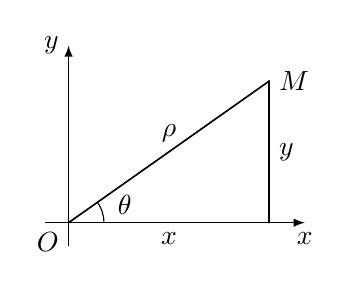
\begin{tikzpicture}[>=latex,scale=1.5]
  \draw[thin,->](-0.2,0)--(2.0,0)node[below]{$x$};
  \draw[thin,->](0,-0.2)--(0,1.5)node[left]{$y$};
  \tkzDefPoints{0/0/O,1.7/1.2/M,1.7/0/N}
  \tkzDrawSegments[semithick](O,M M,N)
  \tkzMarkAngle[size=0.3](N,O,M)
  \tkzLabelAngle[pos=0.5](N,O,M){$\theta$}
  \tkzLabelLine[pos=0.5,above](O,M){$\rho$}
  \tkzLabelLine[pos=0.5,below](O,N){$x$}
  \tkzLabelLine[pos=0.5,right](M,N){$y$}
  \node at (1.7,1.2)[right]{$M$};
  \node at (0,0)[below left]{$O$};
\end{tikzpicture}
\end{document}